\documentclass[]{article}

\usepackage{graphicx}
\graphicspath{ {Images/} }
\usepackage{titlesec}
\usepackage{wrapfig}

\titleformat{\subsection}
  {\normalfont\HUGE\bfseries}{\thesection}{1em}{}[{\titlerule[10.0pt]}]

\titleformat{\subsection}
  {\normalfont\Large\bfseries}{\thesection}{1em}{}[{\titlerule[0.8pt]}]

\begin{document}

\section*{IACS-Computes! 2016 Teaching Assistants}

\subsection*{Joel Anderson} 
\begin{wrapfigure}[6]{R}{0.2\textwidth}
\begin{centering}
    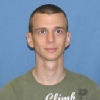
\includegraphics[width=0.2\textwidth]{joel.jpg}
\end{centering}
\end{wrapfigure}
I'm a student in the PhD program in the Applied Mathematics and Statistics department here at Stony Brook University. I use programming every day in my research into numerical methods for relativistic quantum chemistry. I took my first programming course (in Python!) my senior year in high school, and now I primarily program in C++.

\subsection*{Connor Behan} 
\begin{wrapfigure}[6]{R}{0.2\textwidth}
\begin{centering}
    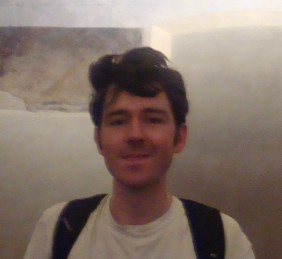
\includegraphics[width=0.2\textwidth]{connor.jpg}
\end{centering}
\end{wrapfigure}
I'm a grad student in Stony Brook's Department of Physics and Astronomy with a hobby of testing patches for a number of random Linux programs. Working with Leonardo Rastelli, I am studying the interplay between quantized fields and various phase transitions in matter, \textit{e.g.} solid to liquid or paramagnetic to ferromagnetic. A program I developed to make this task easier is PyCFTBoot, written in Python. 


\subsection*{Panu Sam-Ang} 
\begin{wrapfigure}[4]{R}{0.2\textwidth}
\begin{centering}
    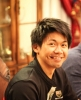
\includegraphics[width=0.2\textwidth]{panu.jpg}
\end{centering}
\end{wrapfigure}
I am a PhD student in the Department of Applied Mathematics and Statistics. My research advisor is Dr. Matthew Reuter. I work in the field of modeling electron transport through molecular junctions. I am from Thailand.
\vspace{0.5 in}

\subsection*{Bryan Sundahl} 
\begin{wrapfigure}{R}{0.2\textwidth}
\begin{centering}
    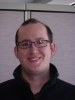
\includegraphics[width=0.193\textwidth]{bryan.jpg}
\end{centering}
\end{wrapfigure}
I'm a graduate student in Applied Math and Statistics here at Stony Brook University, working in the lab of Robert Harrison. My research involves creating software to model the response of molecules to external perturbations (\textit{e.g.} lasers).  Python is the main tool in my analysis of these models. 

\end{document}
